\documentclass[11pt]{article}
\usepackage[utf8]{inputenc}
\usepackage[toc,page]{appendix}
\usepackage{microtype}
\usepackage{fullpage}
\usepackage{multirow}
\usepackage{tocloft}

\usepackage{minted}
\setminted[]{linenos, numbersep=5pt, frame=lines}

\usepackage{parskip}
\setlength{\parindent}{0em}
\setlength{\parskip}{1em}

\usepackage{array}
\newcolumntype{L}{>{\centering\arraybackslash}m{1.2in}}
\newcolumntype{M}{>{\centering\arraybackslash}m{0.85in}}
\usepackage{tablefootnote}

\usepackage[affil-it]{authblk}
\usepackage{amsfonts, amssymb, amsmath}

\usepackage{wrapfig}
\usepackage{graphicx}
\graphicspath{ {./images/} }

\usepackage{float}

\usepackage[backend=biber]{biblatex}
\addbibresource{sources.bib}
% Use the followign Command to validate *.bib file: biber --tool --validate-datamodel qualifying_exam_paper.bib

\title{Improving Emotion Detection through Real-Time Translation of Text to ML Models Trained in Different Languages}

\author{Richard Hoehn%
	\thanks{Electronic address: \texttt{rhoehn@mtmail.mtsu.edu}; corresponding author}}
\affil{Middle Tennessee State University}

\author{Dr. Jaishree Ranganathan%
	\thanks{Electronic address: \texttt{jaishree.ranganathan@mtsu.edu}}}
\affil{Middle Tennessee State University}

\begin{document}

\maketitle

\begin{abstract}
This Qualifying Exam\footnote{PhD students of MTSU Computational and Data Science program are required to complete a Qualifying Exam in their first year in the program.} research paper investigates the potential of improving Emotion Detection (ED) through real-time translation of text to multiple Machine Learning (ML) models trained in different languages. Our research focused on  English and German datasets. This research aims to address the challenges posed by the lack of comprehensive labeled datasets and language fragmentation in ED analysis research and projects, essence the lack of data to better train ML models is trying to be addressed. 

By extending an original English language dataset with a translated dataset from German to English the training data (extended dataset) become larger and the hope is that better prediction rates can be achieved in ED analysis applications due to ML training having more data for learning. Furthermore, translating English to German to extend the German dataset and training another ML model using PySpark and accessing both models in real-time by a simple RESTful API may improve the prediction rates by dual processing a sentence at the same time.

In order to present the results presented both orally to the MTSU's Computational Data \& Science Committee and within this paper labeled datasets both in English and German were collected, translated, and two ML models built that can be accessed via an API to get a prediction on an input (POST or GET) sentence both in German or English.

Sadly the research and results point to the realization that extending the datasets by translation did not improve prediction rates of English or German. Some minor gains can be achieve by accessing both English and German models at the same time via the RESTful API but unfortunately the benefits may not really support the efforts.
\end{abstract}
\clearpage

\tableofcontents

\clearpage
\section{Introduction}

Emotion detection has gained significant interest in recent years as a means to understand human behavior and improve communication effectiveness. By analyzing text, speech or facial expressions, these detection processes try to accurately identify and classify emotions expressed by individuals or groups, often times in real-time.

By employing a variety of ED processes, including natural language processing (NLP) and machine learning (ML), applications with the right amount of data can detect emotions with high precision. These ED systems find applications in diverse fields, such as sentiment analysis, customer feedback analysis, voting and news stances, and mental health monitoring, which all aim at contributing to a deeper understanding of human emotions and their impact on various aspects of life.

\subsection{Human Emotion as a Theoretical Framework}

The concept and number of emotions can vary depending on the theoretical framework or model being considered. One well-known model is the Plutchik's Wheel of Emotions Figure \ref{fig:plutchik-wheel}, which proposes eight (8) primary emotions and their contrasting pairs. In this research paper we will be focusing on the basic eight emotions and not on their sub-emotions or contrasting pairs. This allows the ML models being trained and built to be a multi-classification model with eight label options.

Listed below are the eight primary emotions according to the Plutchik's Wheel of Emotions \cite{Tromp} that we will be focusing on both in English and German, a detailed reference of emotions used in this research can be found in Table \ref{table:dataset_labels} on page~\pageref{table:dataset_labels}.

\begin{itemize}
\item Happiness: A feeling of Joy (Fun), contentment, or delight.
\item Sadness: A state of unhappiness, sorrow, or grief.
\item Anger: An intense emotional response associated with feelings of displeasure, frustration, or hostility.
\item Worry: An emotional response triggered by perceived threats or danger, often associated with anxiety or terror.
\item Surprise: A sudden and unexpected reaction to something unusual or startling.
\item Disgust and/or Hate: A strong aversion or revulsion towards something unpleasant, offensive, or repulsive.
\item Trust and/or Love: A sense of reliance, confidence, or faith in someone or something.
\item Enthusiasm: A feeling of excited expectation or eagerness towards future events.
\end{itemize}

\begin{figure}[h]
    \centering
    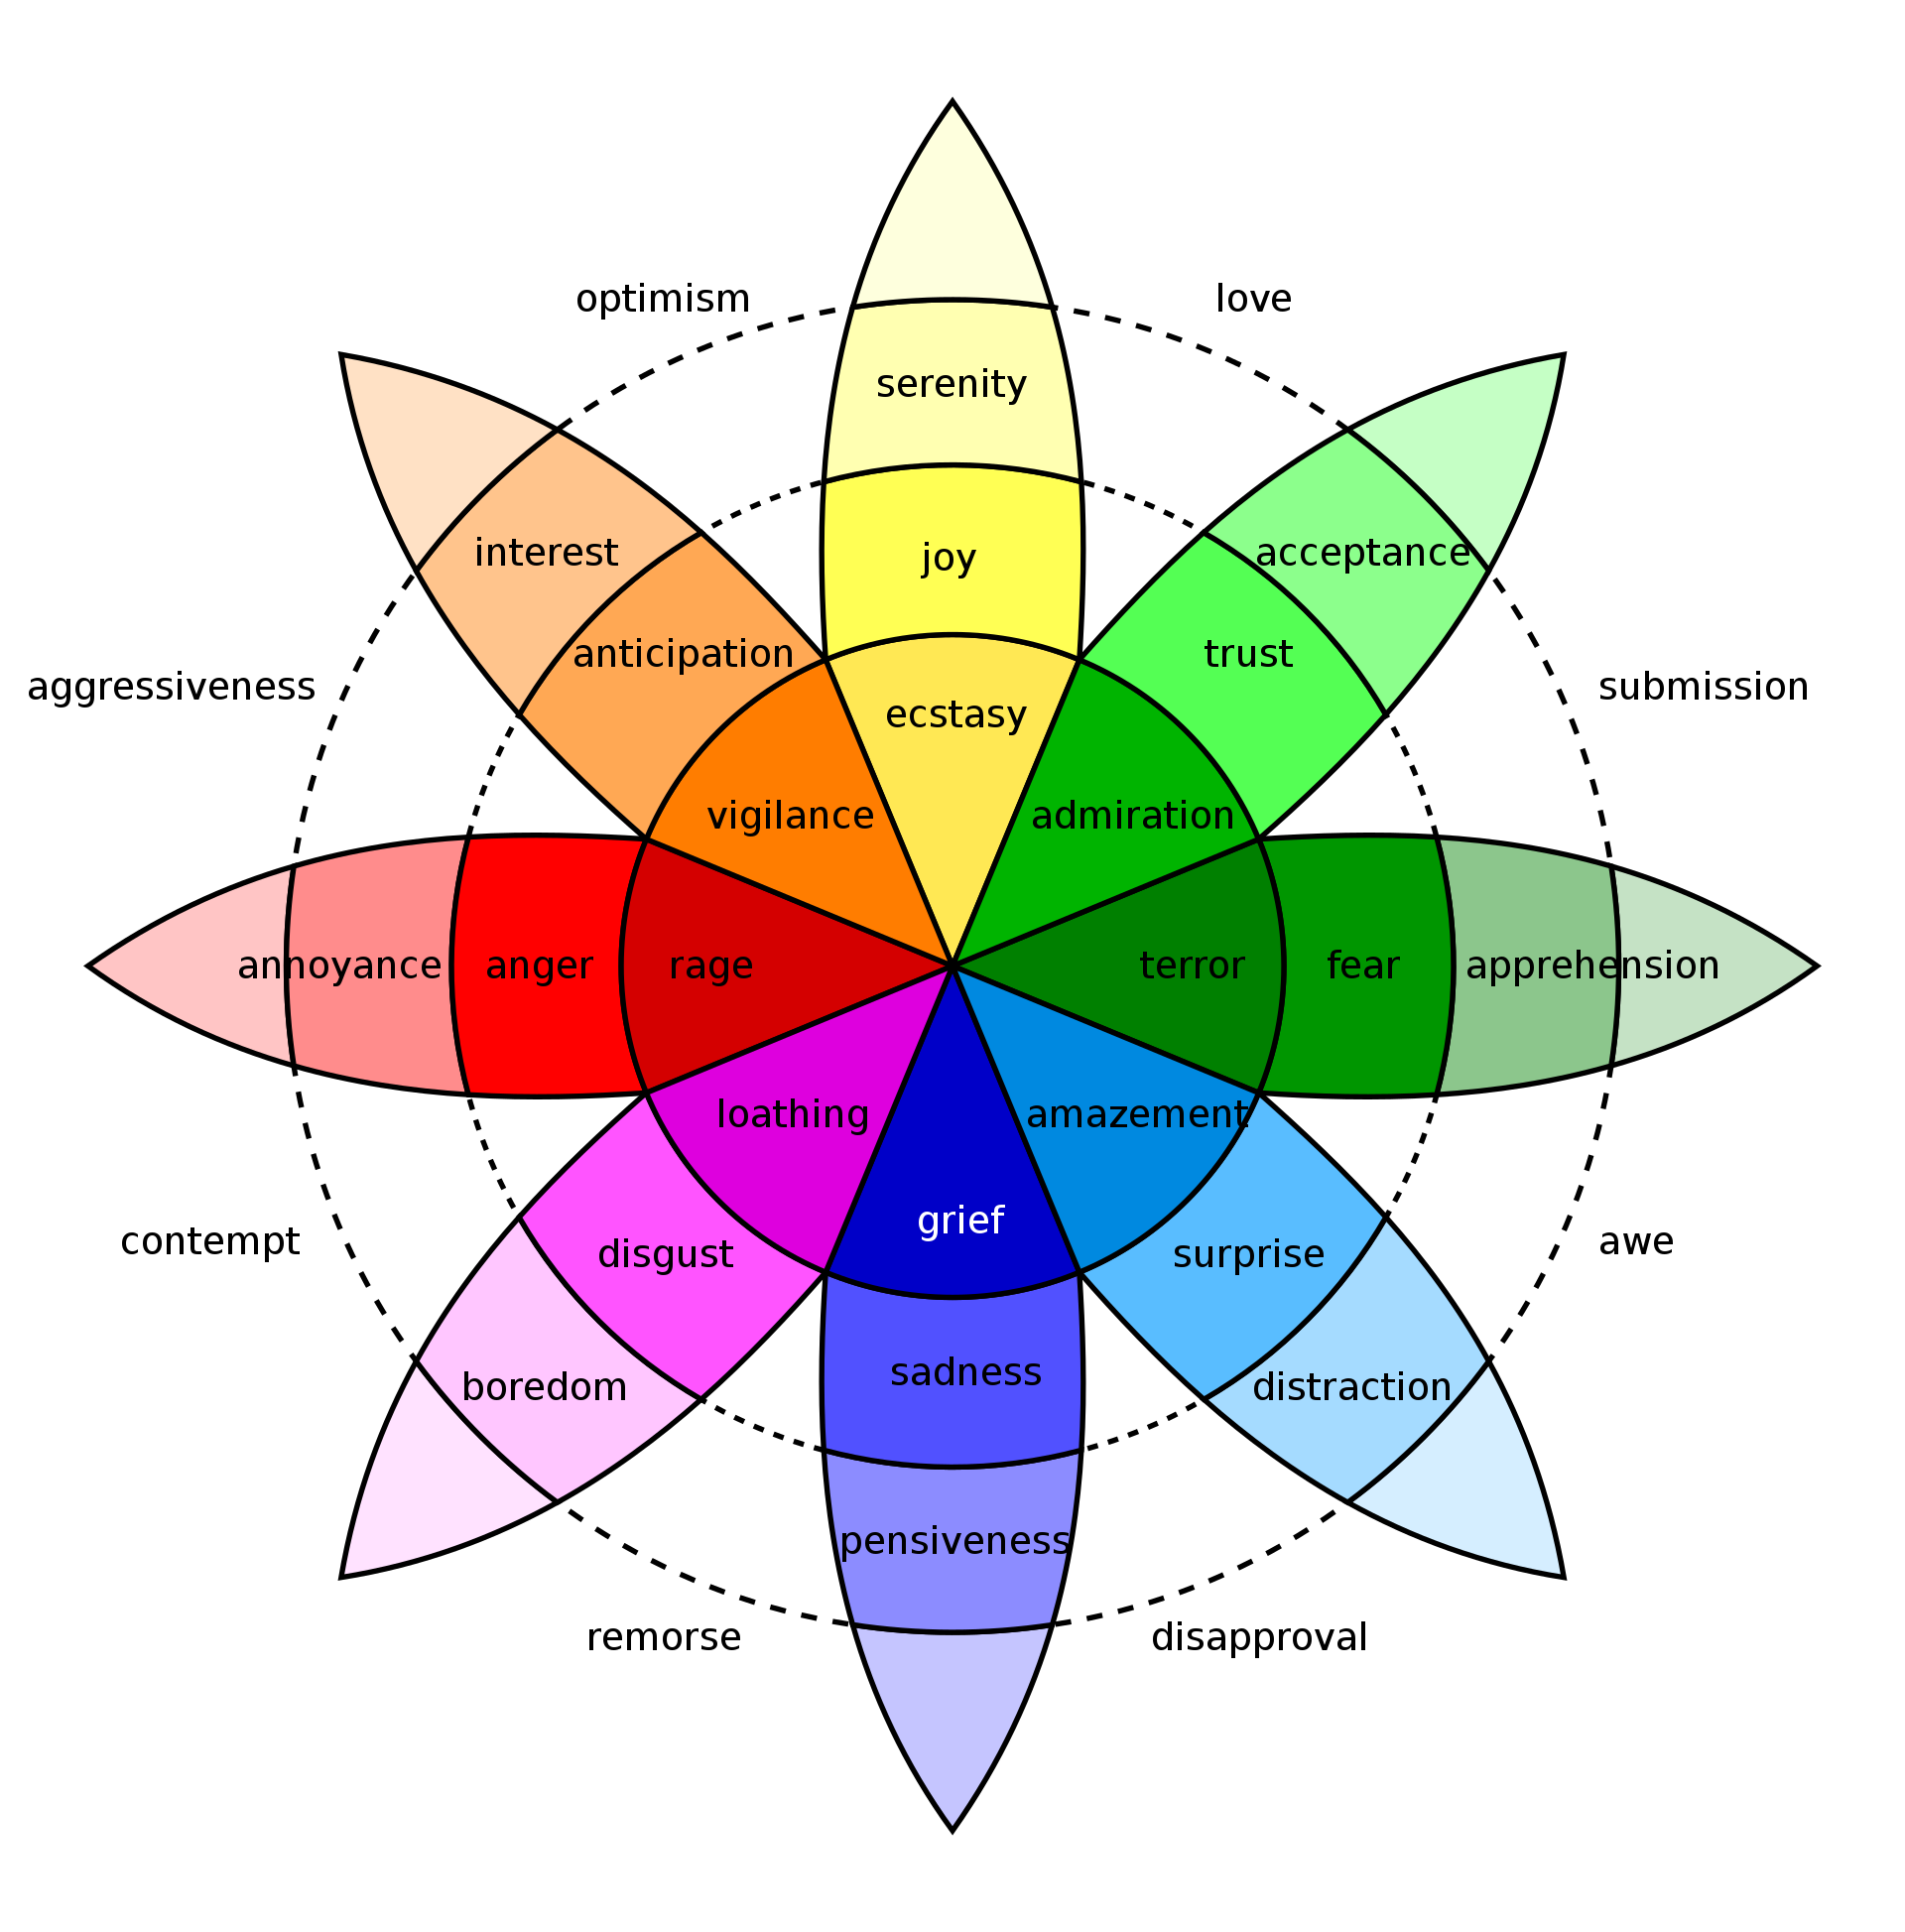
\includegraphics[width=0.4\textwidth]{Plutchik-Wheel}
    \caption{Plutchik Wheel of Emotions}
    \label{fig:plutchik-wheel}
\end{figure}

It's important to note that emotions are complex and multifaceted, and different emotion models or frameworks may propose alternative categorizations or variations in the number of primary emotions. However for the scope of this research project the most common eight (8) emotions are used as described above. This allows the ML models being trained and built to be a multi-classification model with eight label options.

By aligning the emotional labels across the English \cite{english-dataset-twitter} and German \cite{german-dataset-cheese} datasets that are being used in this research all eight listed above were used. Details on the linkage of the two datasets and their counts are described in Section \ref{sec:data-procurement-process} with an emphasis on Table \ref{table:dataset_labels}'s cross reference on page~\pageref{table:dataset_labels} of German and English languages.

\subsection{Significance of Emotion Detection in Machine Learning}
Emotion Detection (ED) analysis in Machine Learning (ML) models has gained significant attention due to its potential applications in various fields, including customer sentiment analysis, stance detection in regard to a specific targets such as news and voting\cite{mascarell-etal-2021-stance}, mental health monitoring\cite{Colonnello}, and human-computer interactions (chatbots\cite{chatbot-cognitive-awareness}) to just name a few.

By accurately identifying and understanding emotions from text data, ML applications can assist in improving user experiences, decision-making processes, and overall human-machine interactions in a positive manner\cite{Colonnello, mascarell-etal-2021-stance}.

As an example, the primary goals of chat-bots are entertainment, social contact, and novelty interaction, with a strong emphasis on productivity, scale-ability and cost reductions. In chat-bots, there has been a immense requirement to simulate human-like characteristics and behavior during human-machine interactions\cite{emotion-detection-literature-review}. Per Kusal et al. \cite{chatbot-cognitive-awareness} these chat-bots also improve customer engagement by offering friendliness, comforters, flexibility, and efficient assistance. Chat-bots should provide customers with more engaging responses, directly addressing their issues or questions. The goal of deploying ED applications is for users perceive chat-bots as companions rather than simple assistants, which in turn helps the overall process of getting to a positive result. Per Adikari et al. the majority of user requests are emotional rather than informative; therefore the need that chat-bots gain the capacity to respond emotionally to customers due to machine learning and sentiment analysis evolution\cite{chatbot-cognitive-awareness} is very important and yields for many applications that employee ED a way to improve interactions with machines.

\begin{quote}
    I usually know almost exactly how I feel. The problem is, I just can’t tell anyone.
    \flushright -- Meg Cabot
\end{quote}

Due to the before mentioned wide scope of uses for ED this field of research and the work to advance it provides significance and importance in enabling machines to comprehend and respond appropriately to human interactions. This in turn contributes to the advancement of artificial intelligence, natural language processing (NLP) and in many cases the utilization of text-to-speech applications most all of us in today's society use and rely on \cite{ai-framework-detection-emotions} to go about our daily lives.

Lastly, in Chen et al.\cite{research-emotion-recognition-for-online-learning} paper based on emotion detection for online learning, it states interestingly that with emotion recognition research, we need to focus on accuracy and real-time performance in order to apply ED based on physiological signals to solve practical problems; the key part of their claim is that in order for ED to be practical, real-time methods needs to be used and deployed for maximum results.

\subsection{Challenges: Lack of Labeled Datasets and Language Fragmentation}
Emotion Detection is an immensely growing field, however unlike Sentiment Analysis (SA) the availability of large datasets for training purposes of ML models is much smaller \cite{ACLU-ED-Data, ai-framework-detection-emotions}. The primary reason of the lack of data stems from the face that emotion detection data requires primarily supervised learning data. In in turn requires time and effort to construct, catalog, and procure,; this all is mostly created and labeled by humans. To compound on the issue of the lack of labeled data; the many datasets that are available are in many cases in multiple languages - not all are in English since emotions that are linked to text are contextual in nature. for this research a a significant amount of time took place to find the German labeled data, which eventually was found online by google searching.

\subsection{Motivation for the research project focusing on extending ED datasets through translation and evaluating the impact on prediction rates}

This paper is significant because an entire industry of automated emotion reading (Text, Image, Video, and Sound) technologies is quickly emerging \cite{ACLU-ED-Data, ACLU-THE-DAWN-OF-ROBOT-SURVEILLANCE}. The market for emotion recognition and detection software is forecast to reach at least \$3.8 billion by 2025 \cite{ACLU-ED-Data, ACLU-THE-DAWN-OF-ROBOT-SURVEILLANCE}. And since ED is already being incorporated into products for purposes such as marketing, robotics, driver safety, customer service, news and stance analysis, and a multiple of others, it is fitting to work on research to solve and / or improve issues in regards to prediction rates and lack of teaching / learning data.

With the before mentioned issues regarding the quantity (lack of) and fragmentation of the ED datasets this research was motivated by finding a way to combine different language datasets into a single set for training processes to improve the predictability of ED. The aim of the research is that by use of translation that the predictability of ED can be improved by extending an English dataset with translations from German and also process look-ups in real-time language conversion and processing.

\subsection{Objectives \& Scope of the Research}

The research project aims at answering the following research questions:

\begin{itemize}
\item Can by translating English data to German and extending an original German dataset increase the predictability of German ED model?
\item Can by translating German data to English and extending an original English dataset increase the predictability of English ED model?
\item Can by translating in real-time an input to multiple languages improve the predictability based on the combined output of two models that were trained in English and German to better the prediction results.
\end{itemize}

With these three (3) objectives our approach will be to procure, translate, train, and evaluate benefits of extending datasets by translation to improve emotion detection. 

\clearpage
\section{Literature Review}
To ensure comprehensive coverage of the latest developments and research in emotion detection and analysis for this research paper, consideration and review was only given to incorporating research papers and online news articles that were published after the year 2015, thereby providing an up-to-date perspective on the subject matter at hand.

We believe by implementing the 2015 boundary, our methodology and results aim to provide a more up-to-date outlook on the subject matter at hand and what areas the emotion detection field is moving in with respect to machine learning research, applications and processes.

\subsection{Emotion Detection Importance and Diverse Populations}
Emotion Detection (ED) holds significant importance in various domains, including psychology, social sciences, and human-computer interaction. It enables the analysis of human emotions at scale, providing valuable insights into individual and collective emotional states both in real-time but also as a type barometer for measuring sentiments from the past versus the current time. In Chowanda et al. paper\cite{CHOWANDA-2021821} they believe that "Emotions hold a paramount role in the conversation, as it expresses context to the conversation.", this means that emotions are a part of a conversation and with that are needed to ensure valid analysis of a conversation.

Furthermore Kapoor et al. \cite{KAPOOR2023120882} states that, emotions can differ across age groups, genders, cultures, and languages. Including data from diverse populations helps in developing inclusive and culturally sensitive ED models. It ensures that the models are not biased towards specific groups and can accurately detect emotions in a wide range of individuals.

\subsection{Lack of Labeled Datasets and Fragmentation caused by Different Languages}
The lack of diverse and large-scale data hinders the development and training of accurate ED models, limiting their effectiveness and general ability across different contexts and populations. In recent research, efforts have been made to address these limitations by exploring new techniques for emotion detection.

For instance, a study by Kapoor\cite{KAPOOR2023120882} et al. proposes analyzing the entire spectrum of the language source to predict emotional changes. This provided some help, but quickly established itself as time consuming task and need of expertise in the subject matters that could not outweigh the results. Overcoming the scarcity of labeled datasets and embracing innovative approaches like the before mentioned study by Kapoor\cite{KAPOOR2023120882} et al. and their analysis can contribute to the advancement of ED research. Such advancements hold the potential to enhance the accuracy and applicability of emotion detection models, enabling a deeper understanding of human emotions and more effective responses in various domains, although the cost of such might be prohibitive at this time.

In addition, the paper by Mascarell\cite{mascarell-etal-2021-stance} et al. states that unlike images language operate very differently, therefore the lack of labeled datasets poses a significant challenge in text-based Emotion Detection (ED) analysis as it limits the availability of reliable training data for ML models. This scarcity hampers the model's ability to learn and generalize emotions effectively.

And lastly, a paper by Kusal et al. further stipulates \cite{kusal} that the fragmentation caused by different languages further exacerbates the issue, as it reduces the size and diversity of data available for training, resulting in limited cross-lingual generalization and potentially biased models.

Overcoming these challenges, lack of data and language fragmentation, is crucial for advancing emotion detection and analysis research for improving the accuracy, speed, and applicability of ML models across various languages and cultures.

\clearpage
\section{Methodology}

\subsection{Data procurement process of ED datasets in English and German}
\label{sec:data-procurement-process}
The data procurement was relatively straight forward and in essence entailed using Google search terms for the Emotion Detection in English and German text languages. Some of the main German data was obtained from the dataset built by ETH's Emotion and Stance Detection for German Text \cite{mascarell-etal-2021-stance} which also hosts a good website with their findings \footnote{https://mtc.ethz.ch/research/natural-language-processing/emotion-stance.html}. The English dataset was downloaded from Kaggle \footnote{https://www.kaggle.com/datasets/pashupatigupta/emotion-detection-from-text} based on Tweets collected in 2021. The English dataset contains over 38,000 tweets and their corresponding emotion labeled. Unfortunately the German dataset only contains over 2,000 sentences and their respective emotions associated. this imbalance of the two dataset sizes will be corrected in the subsequent sections.

\begin{table}[h!]
\centering
\begin{tabular}{ | c | c | c | }
    \hline
    \multicolumn{3}{|c|}{File Details} \\
    \hline
    Name & Row Count & Type \\
    \hline
    English & 38,000 & CSV  \\
    German  &  2,500 & JSON \\
    \hline
\end{tabular}
\caption{File details of English \& German data.}
\label{table:file-details}
\end{table}

An important part of the process is to make sure we match the English emotions to those of the German language emotions. Since the two languages are dissimilar we opted to match exact emotions to each other that can be seen in Table \ref{table:dataset_labels} below.

\begin{table}[h!]
\centering
\begin{tabular}{ | c c | c c | c | }
    \hline
    \multicolumn{5}{|c|}{Emotion Datasets Labels} \\
    
    \hline
    \multicolumn{2}{|c|}{English} & \multicolumn{2}{c|}{German} & \multirow{2}{*}{Used} \\
    Name & Count & Name & Count \\
    \hline
    Boredom    &  179 & ---           & --- & NO  \\
    Love       & 3842 & Vertrauen     & 316 & YES \\
    Relief     & 1526 & ---           & --- & NO  \\ 
    Fun        & 1776 & ---           & --- & NO  \\
    Hate       & 1323 & Ekel          &  29 & YES \\
    Neutral    & 8638 & Unklar        & 314 & YES \\
    Anger      &  110 & Ärger         & 226 & YES \\
    Happiness  & 5209 & Freude        & 140 & YES \\
    Surprise   & 2187 & Überraschung  & 369 & YES \\
    Sadness    & 5165 & Traurigkeit   & 184 & YES \\
    Worry      & 8459 & Angst         & 154 & YES \\
    Enthusiasm &  759 & Antizipation  & 774 & YES \\
    Empty      &  827 & ---           & --- & NO  \\
    \hline
\end{tabular}
\caption{Dataset of English \& German and their respective label counts.}
\label{table:dataset_labels}
\end{table}

Details on how we formatted the the two (English and German) datasets to each other can be viewed in the Appendix \ref{appendix:dataset_english} and \ref{appendix:dataset_german}

The processing of two ED datasets to be synchronized to the emotion is important. The first will be in English and the second in German. Each dataset will be translated into the other’s language for extending purposes. And each row will hold the English and German sentence. As an example Figure \ref{fig:dataset-extension} depicts the original English dataset will be extended by the translated German dataset. By this simple process the English dataset got larger for training purposes.

\begin{figure}[h]
    \centering
    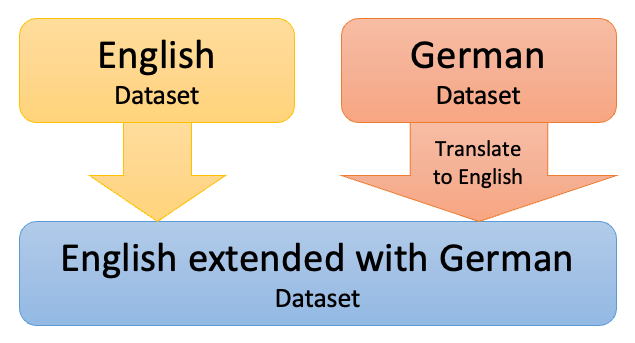
\includegraphics[width=0.4\textwidth]{Dataset-Extension}
    \caption{Example of English dataset extension by translating from German.}
    \label{fig:dataset-extension}
\end{figure}

The reason for selecting German in this research project was based on the author\footnote{Richard Hoehn} being fluent in English and German and hence being able to easily traverse the two languages while working on the code for dataset translations and formatting. It was much easier to create the emotion cross reference Table \ref{table:dataset_labels} and also check the translation results due to the dual language benefit.

Once the two datasets have been translated, we now extend the original language dataset with the translated one.By this approach we are in essence extending the original datasets to create a larger one with the foreign language data. With both extended datasets we can now train our ML models for English and German.

\subsection{Development of a translation application for converting different languages into English and vice versa}
Translation of the emotion datasets was performed with Google Translator based on the Medium article\cite{Nidhaloff_how_to_translate_text_with_python} in which the author describes options for simple API translations. Google Cloud Translation was use mainly due to it's free nature and ease of use for this project. There are however many other text based API translation services that could have been used and might yield in some circumstance even better results.

As an example the following is a brief introduction to Google Translator's API with the code snippet below depicting the ease of use to translate text via an API.

\begin{quote}
\begin{minted}[samepage, fontsize=\small]{python}
#
# Using Deep Translator to leveage Google Translate
# Link: https://cloud.google.com/translate/docs/reference/libraries/v2/python
from deep_translator import GoogleTranslator

sentence = 'Chocolate milk is so much better through a straw.'

translated = GoogleTranslator(source='auto', target='de').translate(sentence)
print(translated) # Schokoladenmilch schmeckt durch einen Strohhalm viel besser.

translated_back = GoogleTranslator(source='auto', target='en').translate(translated)
print(translated_back) # Chocolate milk tastes much better through a straw.

\end{minted}
\end{quote}

Based on the above translation example the CSV (English) and JSON (German) datasets were individually loaded, parsed, and translated to their respective counter-part languages. Details of the application can be found in the Appendix \ref{appendix:dataset_english} for English and Appendix \ref{appendix:dataset_german} for the German processing. We decided to only use 1,500 rows from each language. This decision was made since the German (DE\footnote{DE = German}) dataset was not much larger than that once filtering and processing was completed. This meant that the English (EN\footnote{EN = English}) dataset was randomly paired down to 1,500 to match that of the German. 

Each translated file now contains four (4) columns that are labeled in Tables \ref{table:pd_de_translated} and \ref{table:pd_en_translated} with the exact same column naming.

\begin{table}[h!]
\centering
\begin{tabular}{ | L | L | L | L | }
    \hline
    \multicolumn{4}{|c|}{File: \texttt{pd\textunderscore de\textunderscore translated.csv}} \\
    \hline
    sentence\textunderscore de &
    emotion\textunderscore de & 
    sentence\textunderscore en & 
    emotion\textunderscore en \\
    \hline
    Original Sentence (feature) &
    Original Emotion (label) &
    Sentence Translated to English & 
    Emotion set by Cross-Reference from German \\

    \hline
\end{tabular}
\caption{German CSV file structure after translation to English}
\label{table:pd_de_translated}
\end{table}

\begin{table}[h!]
\centering
\begin{tabular}{ | L | L | L | L | }
    \hline
    \multicolumn{4}{|c|}{File: \texttt{pd\textunderscore en\textunderscore translated.csv}} \\
    \hline
    sentence\textunderscore en &
    emotion\textunderscore en & 
    sentence\textunderscore de & 
    emotion\textunderscore de \\
    \hline
    Original Sentence (feature) &
    Original Emotion (label) &
    Sentence Translated to German & 
    Emotion set by Cross-Reference from English \\

    \hline
\end{tabular}
\caption{English CSV File structure after translation to German}
\label{table:pd_en_translated}
\end{table}

\subsection{Training Multiple ML models with PySpark}
After the completion of translating and processing the Englsih and German datasets we come to training our models. Using the datasets from Tables \ref{table:pd_de_translated}, \ref{table:pd_en_translated}, and \ref{table:ml_models} that list an approximate $\sim$1,275 and $\sim$2,775 features for training.

It is important to note that in order to accurately test and compare the original and the extended datasets to each other we made sure that the test data was the same. to do this we randomly extracted 15\% of the original datasets (English and German) before extending the original with the translated datasets.

\begin{quote}
\begin{minted}[samepage, fontsize=\small]{python}
#
# Split the English and German Dataframes for Training and Testing
# We are using a 15/85 Split
df_en_train, df_en_test = df_en.randomSplit([0.85, 0.15], seed=2023)
df_de_train, df_de_test = df_de.randomSplit([0.85, 0.15], seed=2023)

# Create the Extended Dataframe with Translated Data
# It is important to add the translated to the training data and not all of it
# Using *df_en_train.columns ensure that the columns are matched with the union
df_en_train_extended = df_en_train.union(df_de.select(*df_en_train.columns))
df_de_train_extended = df_de_train.union(df_en.select(*df_de_train.columns))

\end{minted}
\end{quote}

In Chowanda et al. paper\cite{CHOWANDA-2021821} on Text-based Emotion Techniques multiple algorithms were proposed, our research focused on just three (3) out of the six from the paper since the others had lower prediction rates based on the paper\'s conclusions. The algorithms tested in this research project ranged from the traditional machine learning to deep learning techniques, they are:
 \begin{itemize}

\item \textbf{Na\"ive Bayes:} Per Pujan's paper\cite{naive-bayes-model} on the Na\"ive Bayes model, it classifies and/or assigns the most likely class to a given example based on its feature vector, simplifying the task greatly by assuming that the features are independent given a class. 

\item \textbf{Generalised Linear Model (GLM):} Per Mueller's paper on GLM\cite{glm-model} the Generalized linear models extend the concept of the well understood linear regression model.

\item \textbf{Random Forest Classifier:} Per Schonlau's paper\cite{random-forest-model} on the Random Forest Classifier, they state that random decision forests easily adapt to non-linearity found in the data and therefore tend to predict better than linear regression. More specifically, ensemble learning algorithms like random forests are well suited for medium to large datasets.

\end{itemize}
 
Each of these algorithms used and their results are listed in the Results and Analysis Section \ref{sec:results-and-analysis} below.

 \begin{table}[h!]
\centering
\begin{tabular}{ | L | L | L | L | }
    \hline
    \multicolumn{4}{|c|}{ML Models } \\
    \hline
    Model & 
    Data &
    Rows for Training (85\%) & 
    Rows for Testing (15\%)  \\
    \hline
    A &
    English Original &
    1,275 & 
    225 \\
    \hline
    B &
    English Extended By German &
    2,775 & 
    225 same as Model "A" \\
    \hline
    C &
    German Original &
    1,275 & 
    225 \\
    \hline
    D &
    German Extended By English &
    2,775 & 
    225 same as Model "C" \\
    \hline
\end{tabular}
\caption{ML Models and their respective settings}
\label{table:ml_models}
\end{table}

The results of the testing resulted in some interesting parts that can be viewed in Table \ref{table:ml-prediction-result-versus-test-data}. We grouped the label by count from the test data (both English and German) and compared the predicted result counts to those. It became very clear that there was a strong bias on the GLM (Linear Regression) model that essentially proposed that all sentences evalued to the same output both in English and German.

\begin{table}[h!]
\centering
\begin{tabular}{ | M | M | M | M | M | M | }
    \hline
    \multicolumn{6}{|c|}{ML Models Test versus Test Result Counts} \\
    \multicolumn{6}{|c|}{} \\
    \multicolumn{6}{|c|}{English} \\
    \hline
    ID & 
    Label &
    Test Data &
    NB Res & 
    GLM Res  &
    RFC Res \\
    \hline
    0 & boredom     &  0 & 25 \tablefootnote{In the NB a result that cannot be matched is a zero label} &   0 &   0 \\
    1 & love        & 26 &  8 &   3 &  11 \\
    2 & Relief      &  0 & 33 &   0 &   0 \\
    3 & Fun         &  0 &  5 &   0 &   0 \\
    4 & hate        &  9 & 31 &   0 &   0 \\
    5 & neutral     & 50 & 21 & 152 & 101 \\ 
    6 & anger       &  0 & 36 &   0 &   0 \\
    7 & happiness   & 39 & 44 &   5 &  17 \\
    8 & surprise    & 10 &  9 &   0 &   1 \\
    9 & sadness     & 29 &  0 &   2 &  19 \\
    10 & worry      & 46 &  0 &  50 &  63 \\
    11 & enthusiasm &  3 &  0 &   0 &   0 \\
    \hline
    \multicolumn{6}{|c|}{} \\
    \multicolumn{6}{|c|}{German} \\
    \hline
    ID & 
    Label &
    Test Data &
    NB Res & 
    GLM Res  &
    RFC Res \\
    \hline
    0 & boredom     &  0 & 34 &   0 &   0 \\
    1 & love        & 25 &  5 &   0 &  13 \\
    2 & Relief      &  0 & 28 &   0 &   0 \\
    3 & Fun         &  0 & 16 &   0 &   0 \\
    4 & hate        &  5 & 16 &   0 &   2 \\
    5 & neutral     & 30 & 24 &   0 &   5 \\ 
    6 & anger       & 23 & 20 &   1 &   7 \\
    7 & happiness   & 10 & 20 &   0 &   5 \\
    8 & surprise    & 24 & 47 &   0 &  11 \\
    9 & sadness     & 12 &  0 &   0 &   2 \\
    10 & worry      &  9 &  0 & 209 &   4 \\
    11 & enthusiasm & 72 &  0 &   0 & 161 \\
    \hline
\end{tabular}
\caption{Prediction Results Count compared to Test Data Label Counts}
\label{table:ml-prediction-result-versus-test-data}
\end{table}

In order for each of the three ML models to be processed at the same time we crated a Jupyter Notebook that starts an Apache PySpark\footnote{PySpark: https://spark.apache.org/docs/latest/api/python/index.html} session that is accessed via the local server running that accepts RESTful API calls with details of the server in Appendix \ref{appendix:code-api-server}.

\subsection{Evaluation Metrics and Methodologies for Measuring the Performance}
\label{sec:evaluation-metrics-and-methodologies}
The evaluation of ML models trained on the English, German and their respective extension datasets is a critical step in assessing their performance and reliability. We chose to use the MulticlassClassificationEvaluator\footnote{URL: https://spark.apache.org/docs/latest/api/python/reference/api/pyspark.ml.evaluation.MulticlassClassificationEvaluator.html} because is a well known tool in the field of natural language processing (NLP) research, specifically in multi-class classification tasks such as emotion detection that has multiple labels associated with it; in our case eight (8) see Table \ref{table:dataset_labels} on Page \pageref{table:dataset_labels}. Generally this evaluator is used to evaluate the performance of machine learning (ML) models, using transformer-based architectures like BERT, RoBERTa, or DistilBERT\cite{Sanh2019-DistilBERT-AD}, with DistilBERT\cite{Sanh2019-DistilBERT-AD} being the one we used in this research project.

The MulticlassClassificationEvaluator provides the essential evaluation metrics, including accuracy, Precision (eq: \ref{eq:precision}), Recall (eq: \ref{eq:recall}), and F1 Score (eq: \ref{eq:f1-score}) for ED classifications. These metrics provide valuable insights into a model's ability to correctly classify emotions across multiple classes and languages. Our research project is no different and the following measurements were used for our analysis:
\begin{itemize}

\item \textbf{Accuracy:} Accuracy measures the overall correctness of the emotion predictions made by the model. It is calculated as the ratio of correctly classified instances to the total number of instances in the dataset.

\item \textbf{F1 Score:} Precision represents the proportion of correctly predicted emotions among all instances predicted as a specific emotion with respect to the labels. Recall measures the proportion of correctly predicted emotions among all instances that truly belong to a specific emotion. With these two the F1 Score ($F1_{Score}=\frac{\text{Precision} \times \text{Recall}}{\text{Precision} + \text{Recall}}$) combines precision and recall into a single metric, providing a balanced evaluation.

\end{itemize}

While evaluating the models we focused on the Accuracy and the F1 Score to illustrate the prediction results of the original versus extended datasets, and also compared the different algorithms to each other. As an added example simply using the accuracy to evaluate a model can be miss-leading and therefore in our case using the F1 Score, that is directly correlated to the Precision (eq: \ref{eq:precision} and Recall (eq: \ref{eq:recall}) is immensely important to understanding the ones models and finding the best of for the task of Emotion Detection using Original and Extended datasets.

\subsection{Written \& Oral Presentation of Research Finding}
In conclusion of the project a research paper and oral presentation is required to pass the  MTSU Computation Data Science PhD Qualifying Exam. The listing of all the datasets used, code for the application, and details of the research project process in this research paper is openly available and hosted on a GitHub repository, allowing for easy access, reproducible, and collaborative engagement with the research findings. The repository is open and available under: \texttt{https://github.com/richardhoehn/mtsu.coms.qualifying-exam}\cite{Hoehn_Improving_Emotion_Detection_2023}. In addition of all the code being listed in a public repository the paper was comprised and build using \LaTeX\footnote{LaTeX UR: https://www.latex-project.org/}.

Using \LaTeX\;for this paper provides numerous benefits, some of which are portability, source control (due to plain-text nature), bibliography management, and last but not least the ability to write clean mathematical equations. 

\clearpage
\section{Results and Analysis}
\label{sec:results-and-analysis}
The following section lists the prediction rates of training and testing of the original and extended datasets both in English and German. Overall results seem to indicate that there was no measurable benefit and even negative outcomes based on adding the extended data for Emotion Detection. In the below sub sections details on the results are listed by the common standards of using the below equations \ref{eq:accuracy}, \ref{eq:precision}, \ref{eq:recall}, and \ref{eq:f1-score} for Accuracy, Precision, Recall, and the F1 Score. It should be noted that ED is a Multi-class classification problem, which means that the machine learning process assigns the predictions from the sentence data to one of several predefined emotion categories (see Table \ref{table:dataset_labels}).

\subsection{Prediction Results of Original \& Extended Datasets}
Overall the prediction results from the trained models is disappointing. Using the Random Forrest Classifier described in Section \ref{sec:evaluation-metrics-and-methodologies} provided the best prediction results based on a combination of the Accuracy and the F1 Score. It should be noted although the accuracy may be slightly better on the GLM models for both English and German, if one reviews the F1 Score, the RFC model performs better.

Oddly, the prediction results with the extended data where lower than using the original (non-extended) data for training. In the analysis and conclusions section \ref{sec:analysis-of-impact-of-extending-datasets} below details on why this may be the case are discussed in detail.

\subsubsection{Formulas and Equations used in Analysis}
The accuracy (eq: \ref{eq:accuracy}) of any machine learning model is a clear and easily comprehend-able way to understand the performance of a model. However, it is important to consider the context and potential trade-offs with other metrics, as high accuracy alone might not capture the full picture of a model's performance.
\begin{equation}
Accuracy = \frac{TP+TN}{TP+TN+FP+FN}
\label{eq:accuracy}
\end{equation}

The Precision (eq: \ref{eq:precision}) focuses in detail on the accuracy of positive predictions (TP)\footnote{Positive Predictions = TP (True Positive)} made by the model. Per Google Cloud's definition the precision answers: What proportion of positive predictions where actually correct?
\begin{equation}
Precision = \frac{TP}{TP+FP}
\label{eq:precision}
\end{equation}
Since our project is a multi-class classification project we will need to actually use Micro Averaging for the Precision. With this in mind we extend our simple equation \ref{eq:precision} of precision to incorporate micro averaging is illustrated in equation \ref{eq:precision_micro_avg}.
\begin{equation}
Precision_{MicroAvg} = \frac{(TP_1 + TP_2 + \ldots + TP_n)}{(TP_1 + TP_2 + \ldots + TP_n + FP_1 + FP_2 + \ldots + FP_n)}
\label{eq:precision_micro_avg}
\end{equation}

The Recall (eq: \ref{eq:recall}) focuses on the in detail on the accuracy of positive predictions\footnote{Negative Predictions = FN (False Negative)} made by the model. Per Google Cloud's definition: The recall attempts to answer: What proportion of actual positives.

\begin{equation}
Recall = \frac{TP}{TP+FN}
\label{eq:recall}
\end{equation}

Since our project is a multi-class classification project we will need to actually use Micro Averaging for the Recall in a similar fashion to how we used it on Precision. With this in mind we extend our simple equation \ref{eq:recall} of recall to incorporate micro averaging is illustrated in equation \ref{eq:recall_micro_avg}.

\begin{equation}
Recall_{MicroAvg} = \frac{(TP_1 + TP_2 + \ldots + TP_n)}{(TP_1 + TP_2 + \ldots + TP_n + FP_1 + FP_2 + \ldots + FP_n)}
\label{eq:recall_micro_avg}
\end{equation}

The F1 score (eq: \ref{eq:f1-score}) in our project is important to assess the balance between precision and recall. In addition, the F1 score is especially relevant in multi-class classification scenarios where there are more than two classes.

\begin{equation}
F1_{Score} = \frac{2*Precision*Recall}{Precision+Recall}
\label{eq:f1-score}
\end{equation}

Lastly, we used micro averaging for the Recall, Precision, and F1 Score due to fact it give each label (Emotion see Table \ref{table:dataset_labels}) equal weight regardless of the class label and the number of labels counted.

\subsubsection{English Dataset Results}
\label{sec:english-dataset-results}
The Table \ref{table:en_testing_results} lists the results of all three ML models, their accuracy and F1 Score based on the English original and extended datasets. The improvements from the original and extended datasets are listed in the last column. In all cases the improvement to using the extended datasets was negative.

\begin{table}[h!]
\centering
\begin{tabular}{ | L | M | M | M | M | M | }
    \hline
    \multicolumn{6}{|c|}{Results of English Dataset} \\
    \hline
    &
    \multicolumn{2}{c|}{Original Dataset} &
    \multicolumn{3}{c|}{Extended Dataset} \\
    & Accuracy & F1 Score & Accuracy & F1 Score & Improvement \\
    \hline
    Random Forrest & 
    29.72\% &
    25.83\% & 
    21.23\%  &
    19.43\% &
    -28.56\% \\
    \hline
    Na\"ive Bayes & 
    5.66\% &
    6.92\% & 
    3.77\%  &
    4.14\% &
    -33.39\% \\
    \hline
    GLM (lr) & 
    32.08\% &
    23.68\% & 
    25.47\%  &
    16.19\% &
    -19.95\% \\
    \hline
\end{tabular}
\caption{Model Testing Results on English Dataset}
\label{table:en_testing_results}
\end{table}

\subsubsection{German Dataset Results}
\label{sec:german-dataset-results}
The Table \ref{table:de_testing_results} lists the results of all three ML models, their accuracy and F1 Score based on the German original and translated from English to German extended datasets. The improvements from the original and extended datasets are listed in the last column. Interestingly the Random Forrest Classifier was the only negative improvement whereas the GLM and Naive Bayes models had improvements. However it should be noted that the prediction rates are so low in the GLM and Naive Bayes that they should not really be considered improvements.

\begin{table}[h!]
\centering
\begin{tabular}{ | L | M | M | M | M | M | }
    \hline
    \multicolumn{6}{|c|}{Results of German Dataset} \\
    \hline
    &
    \multicolumn{2}{c|}{Original Dataset} &
    \multicolumn{3}{c|}{Extended Dataset} \\
    & Accuracy & F1 Score & Accuracy & F1 Score & Improvement \\
    \hline
    Random Forrest & 
    28.10\% &
    16.84\% & 
    25.71\%  &
    18.56\% &
    -8.50\% \\
    \hline
    Na\"ive Bayes & 
    4.29\% &
    4.31\% & 
    6.67\%  &
    4.21\% &
    +55.48\% \\
    \hline
    GLM (lr) & 
    34.29\% &
    17.57\% & 
    24.76\%  &
    18.27\% &
    -27.79\% \\
    \hline
\end{tabular}
\caption{Model Testing Results on German Dataset}
\label{table:de_testing_results}
\end{table}

The improvements on the accuracy are based on Equation \eqref{eq:improvement} listed below. It is a simple and straightforward way of comparing the Accuracy from the original trained dataset to the extended trained dataset for purposes of comparing the potential benefits of extending the training datasets by translation.

\begin{equation}
Improvement(\%) = \dfrac{(Accuracy_{Ext} (\%) - Accuracy_{Org} (\%))}{Accuracy_{Org}(\%)}
\label{eq:improvement}
\end{equation}

It should be noted that although the improvement values are fairly large negatives those come from the fact that the accuracy is small and in most all cases the accuracy is around the 25 - 30\% values and a change of just a few percent can have a significant impact on the improvement values.

\subsection{Analysis of the impact of Extending Datasets by Translation}
\label{sec:analysis-of-impact-of-extending-datasets}
While extending datasets for machine learning training can often improve\cite{Sarker2021} model performance, it's important to recognize that this approach has its limitations, especially in ML models that can reach a limit on training data. In our case, relying on translation services for dataset expansion might not consistently yield better results when extending the data from translated text. These services, in our case using Google Translate\footnote{Google Cloud Translate URL: https://cloud.google.com/translate} can introduce errors or inaccuracies in translations especially in the context of emotions of a particular text, leading to noisy or incorrect training data. Consequently, the models may learn from erroneous information, which did negatively impact our models performance on the ED tasks.

Specifically in our case of extending the original English and German datasets with translated data seems to indicate that the sentences and structure are not the same and therefore the prediction rates went down as the models got more diluted.

\subsection{Findings and Implications for Improving Emotion Detection}
Based on the improvement results in Sections \ref{sec:english-dataset-results} and \ref{sec:german-dataset-results} it seems that using translation to extend both the English and German datasets resulted in a negative outcomes. The best outcomes were using a simple Linear Regression model on the English and German, however based on the F1 score (EQ \ref{eq:f1-score}) of the Random Forest Classifier it seems to perform the best on both English and German. 

Unfortunately based on the results of extending the data our approach to also using real-time translation for multi-language models 

\subsection{Conclusion and Future Work}
It's crucial to ensure the quality and accuracy of extended data, especially when language translation is involved, to prevent introducing more noise than meaningful information into the training process. Although the research did not garner any significant improvements by translating the German to English as a means on extending the English dataset, it actually made it the prediction results worse.

Future work includes testing and translating different models by using different translation services. Using Google Cloud's translation service was adequate for this research, however there are certainly better translation services that are available but are based on paid subscriptions.

\clearpage
\addcontentsline{toc}{section}{References}
\printbibliography
\clearpage


\addcontentsline{toc}{section}{List of Figures}
\listoffigures
\clearpage


% Appendix Details
\appendix
\section{Appendix -- Dataset Details}
The following details in this appendix are for clarification purposes.
All examples in this appendix are created via PySpark using dataframes.

\subsection{Using PySpark to Load Data}
All example code was created using Jupyter Notebooks creating a PySpark session. The details of setting up such session are below in the code example. All subsequent details are derived from the \texttt{sc}\footnote{sc = Spark Session}.
\begin{minted}[fontsize=\small]{python}
# General Imports
import glob
import shutil

# Setup Spark Session
from pyspark.sql import SparkSession

# Get Spark Functions Needed
from pyspark.sql.functions import col, udf, split, explode

# Get Datatypes needed for DataFrame manipulation
from pyspark.sql.types import IntegerType, StringType

# Setup Spark Session
sc = SparkSession \
        .builder \
        .master("local[*]") \
        .appName("data_clean_up") \
        .getOrCreate()

# Print Spark Version being run
print("Spark V: ", sc.version)
\end{minted}
\clearpage


\subsection{Details on English Dataset}
\label{appendix:dataset_english}
The English dataset is based on tweets\footnote{Tweets from Twitter} that are saved as a \texttt{csv}\footnote{csv = Comma Separated Values} file. The following code was use to filter and process the file for use in this project.
\begin{minted}[fontsize=\small]{python}
# *********************************
# *** English Data Preparations ***
# *********************************

# Load English CSV File into a Dataframe
df_english = sc.read.csv("data/english.csv", header=True, inferSchema=True)
print(f'Count (raw): {df_english.count()}')

# Print Columns
print(f'English Source Columns: {df_english.columns}\n')

# Filter only lavbels that we mathc with the German counter parts
filter_values = ["love", "hate", "neutral", "anger", "happiness", "surprise", "sadness", "worry", "enthusiasm"]
df_english_filtered = df_english.filter(col("sentiment").isin(filter_values))

# Remove unnecessary column
df_english_filtered = df_english_filtered.drop("tweet_id")

# Rename Columns
df_english_filtered = df_english_filtered.withColumnRenamed("sentiment", "emotion_en")
df_english_filtered = df_english_filtered.withColumnRenamed("content", "sentence_en")

# Make sure the column order to the same for both german and english csv files
df_english_filtered = df_english_filtered.select('sentence_en', 'emotion_en')

print(f'Count (filtered): {df_english_filtered.count()}')

# Group By for Details & Count
df_english_grouped = df_english_filtered.groupBy('emotion_en').count()

# Show Groupings and Respetive Counts
print('\nGrouped & Count by "emotion"')
df_english_grouped.show(truncate=0)


# Save Dataframe to CSV
directory_path = 'data/spark_data_parts'
df_english_filtered.coalesce(1).write.csv(directory_path, header=True, mode="overwrite")

file_pattern = 'part-00000*.csv'
file_path = glob.glob(directory_path + '/' + file_pattern)[0]

shutil.move(file_path, './data/data_en.csv')

Count (raw): 40000
English Source Columns: ['tweet_id', 'sentiment', 'content']

Count (filtered): 35692

Grouped & Count by "emotion"
+----------+-----+
|emotion_en|count|
+----------+-----+
|love      |3842 |
|hate      |1323 |
|neutral   |8638 |
|anger     |110  |
|happiness |5209 |
|surprise  |2187 |
|sadness   |5165 |
|worry     |8459 |
|enthusiasm|759  |
+----------+-----+
\end{minted}
\clearpage

\subsection{Details on German Dataset}
\label{appendix:dataset_german}
The German dataset was downloaded from the ETH's\footnote{ETH (German: Eidgenössische Technische Hochschule) or Swiss Federal Institute of Technology} servers via "link" as a \texttt{JSON} file. Since the the file was \texttt{JSON} we will need to filter and explode the file based on teh emotions that are attached to it.
\begin{minted}[fontsize=\small]{python}
# ********************************
# *** German Data Preparations ***
# ********************************

# Load German JSON File into a Dataframe
df_german = sc.read.json("data/german.json")
print(f'Count (raw): {df_german.count()}')

# Print Columns
print(f'German Source Columns: {df_german.columns}\n')


# We Need to "split" the "artice_emotion" column since the ETH team listed
# multiple emotions in one column
# In order to "explode" the column to it's distinct rows
df_german_exploded = df_german.select('*', explode('article_emotion').alias('emotion_de'))

# Rename Column
df_german_exploded = df_german_exploded.withColumnRenamed("title", "sentence_de")

# Remove unnecessary column
df_german_exploded = df_german_exploded.drop("article_id")
df_german_exploded = df_german_exploded.drop("article_stance")
df_german_exploded = df_german_exploded.drop("paragraphs")
df_german_exploded = df_german_exploded.drop("source")
df_german_exploded = df_german_exploded.drop("article_emotion")
df_german_exploded = df_german_exploded.drop("snippet")

# Make sure the column order to the same for both german and english csv files
df_german_exploded = df_german_exploded.select('sentence_de', 'emotion_de')

print(f'Count (filtered): {df_german_exploded.count()}')

# Group By for Details & Count
df_german_grouped = df_german_exploded.groupBy('emotion_de').count()

# Show Groupings and Respetive Counts
print('\nGrouped & Count by "emotion"')
df_german_grouped.show(truncate=0)


# Save Dataframe to CSV
directory_path = 'data/spark_data_parts'
df_german_exploded.coalesce(1).write.csv(directory_path, header=True, mode="overwrite")

file_pattern = 'part-00000*.csv'
file_path = glob.glob(directory_path + '/' + file_pattern)[0]

shutil.move(file_path, './data/data_de.csv')

Count (raw): 1970
German Source Columns: ['article_emotion', 'article_id', 'article_stance', 'paragraphs', 'snippet', 'source', 'title']

Count (filtered): 2568

Grouped & Count by "emotion"
+------------+-----+
|emotion_de  |count|
+------------+-----+
|Vertrauen   |316  |
|Freude      |140  |
|Ärger       |226  |
|Überraschung|369  |
|Traurigkeit |184  |
|Antizipation|774  |
|Unklar      |314  |
|Angst       |154  |
|Ekel        |29   |
|Keine       |62   |
+------------+-----+
\end{minted}
\clearpage


\subsection{Details on Extending \& Translation}
\label{appendix:dataset_translation}
Details on translation and extending the datasets.
\begin{minted}[fontsize=\small]{python}
# **************************************
# *** English <-> German Emotion Key ***
# **************************************


from pyspark.sql.functions import col, udf, split, explode, lit
from pyspark.sql.types import IntegerType, StringType, StructType, StructField, StringType

# Emotion Dictionary English <-> German
# This key/value setup was previsoulsy created for linking purposes
emotion_key = {
    "boredom"    : "---",
    "love"       : "Vertrauen",
    "relief"     : "---",
    "fun"        : "---",
    "hate"       : "Ekel",
    "neutral"    : "Unklar",
    "anger"      : "Ärger",
    "happiness"  : "Freude",
    "surprise"   : "Überraschung", 
    "sadness"    : "Traurigkeit", 
    "worry"      : "Angst",
    "enthusiasm" : "Antizipation", 
    "empty "     : "---",
    "---"        : "Keine",
}

# Create the schema for the DataFrame
schema = StructType([
    StructField("emotion_en", StringType(), nullable=False),
    StructField("emotion_de", StringType(), nullable=False)
])

# Convert the dictionary to a list of tuples
data = [(key, value) for key, value in emotion_key.items()]

# Create the PySaprk DataFrame
df_emotion_key = sc.createDataFrame(data, schema)

df_emotion_key.show()

# Extend the English and German onto the datasets
df_german_exploded = df_german_exploded.join(df_emotion_key, on="emotion_de", how="left")
df_english_filtered = df_english_filtered.join(df_emotion_key, on="emotion_en", how="left")

# New sentence column
df_german_exploded = df_german_exploded.withColumn("sentence_en", lit(None))
df_english_filtered = df_english_filtered.withColumn("sentence_de", lit(None))

df_german_exploded.show()
df_english_filtered.show()


# Using Deep Translator to proxy to Google Translate
from deep_translator import GoogleTranslator


# Define Tranlation Functions
def translate_en_to_de(row):
    translated = GoogleTranslator(source='en', target='de').translate(row["sentence_en"])
    row["sentence_de"] = translated

def translate_de_to_en(row):
    translated = GoogleTranslator(source='de', target='en').translate(row["sentence_en"])
    row["sentence_en"] = translated
    

df_german_exploded.foreach(translate_de_to_en)  

+----------+------------+
|emotion_en|  emotion_de|
+----------+------------+
|   boredom|         ---|
|      love|   Vertrauen|
|    relief|         ---|
|       fun|         ---|
|      hate|        Ekel|
|   neutral|      Unklar|
|     anger|       Ärger|
| happiness|      Freude|
|  surprise|Überraschung|
|   sadness| Traurigkeit|
|     worry|       Angst|
|enthusiasm|Antizipation|
|    empty |         ---|
|       ---|       Keine|
+----------+------------+

+------------+--------------------+----------+----------+-----------+----------+
|  emotion_de|         sentence_de|emotion_en|emotion_en|sentence_en|emotion_en|
+------------+--------------------+----------+----------+-----------+----------+
|   Vertrauen|Adoptiert zu sein...|      love|      love|       null|      love|
|      Freude|Österreichs Verfa...| happiness| happiness|       null| happiness|
|      Freude|Visana gewinnt er...| happiness| happiness|       null| happiness|
\end{minted}
\clearpage
 % Note: SubSection headers are handled within the *.tex file 
\section{Appendix -- Application \& Code Details}
Hello World - Application \& Code Details
\subsection{Application}
\label{appendix:code_application}
Hello World - Application
\clearpage

\subsection{Code Details}
Hello World - Code Details

\subsection{RESTful API Server}
\label{appendix:code-api-server}
The RESTful\footnote{RESTful API is an interface that two computer systems use to exchange information securely over the internet.} API Server will be a simple Python Flask server listening on port \texttt{8080} on the local machine.


\clearpage
 % Note: SubSection headers are handled within the *.tex file 

\end{document}



